% Light!
\documentclass[8pt, a4paper, oneside, twocolumn]{extarticle}
\usepackage{verbatim}  % for multiline comments
\begin{comment}
The options oneside and twoside affect the width of the side margins.  With oneside , which is the default for article, report, and letter, the margins on both  sides  of  every  page  are  equally  wide.   With twoside, Latex distinguishes between an inner and outer  margin.   The  outer  margin  is  substantially wider  and  switches  between  left  and  right.   Even pages have their outer margin on the left, odd pages on the right.  Most books follow this structure and so it should not come as a surprise that the book class default is twoside.
The standard Latex classes (article, report etc) support ten, eleven and twelve point text. These are the commonest sizes used in publishing.
However, for certain applications there may be a need for other sizes.
The extsizes classes (extarticle, extreport, extbook, extletter, and
extproc) provide support for sizes eight, nine, ten, eleven, twelve,
fourteen, seventeen and twenty points.	
Also as we want whole document to have two columns, we gave it as an optimal parameter however if we want a particular page to have two columns, the command \twocolumn starts a new page having two columns. Accordingly, \onecolumn starts a new page with a single column assuming you are in a two column environment as described above. Both commans do not take any arguments. 
The is a way to define the distance between the two columns, use
\setlength{\columnsep}{distance}

If you need a line to separate the columns, the following command will do the job:
\setlength{\columnseprule}{thickness}
\end{comment}
\usepackage{graphicx}
\usepackage[export]{adjustbox}
\usepackage[compact]{titlesec}  % documentation: http://mirror.iopb.res.in/tex-archive/macros/latex/contrib/titlesec/titlesec.pdf  
\usepackage{kotex}
\usepackage[left=0.8cm, right=0.8cm, top=2cm, bottom=0.3cm, a4paper]{geometry}
\usepackage{amsmath}
\usepackage{ulem}
\usepackage{amssymb}
\usepackage{minted}  % syntax highlighting
\usepackage{enumitem}
\setlist{nolistsep}
\usepackage{fancyhdr} % documentation: http://ctan.math.utah.edu/ctan/tex-archive/macros/latex/contrib/fancyhdr/fancyhdr.pdf
\begin{comment}
The pack­age pro­vides ex­ten­sive fa­cil­i­ties, both for con­struct­ing head­ers and foot­ers, and for con­trol­ling their use (for ex­am­ple, at times when LaTeX would au­to­mat­i­cally change the head­ing style in use).
\end{comment}
\usepackage{lastpage}  % just so that we can use \pageref {LastPage}
\usepackage{color, hyperref}
% The lines in the table of contents become links to the corresponding pages in the document by simply adding in the preamble of the document the line
\begin{comment}
\titlespacing{command}{left spacing}{before spacing}{after spacing}[right]
% spacing: how to read {12pt plus 4pt minus 2pt}
%           12pt is what we would like the spacing to be
%           plus 4pt means that TeX can stretch it by at most 4pt
%           minus 2pt means that TeX can shrink it by at most 2pt
%       This is one example of the concept of, 'glue', in TeX
\end{comment}
\usepackage{tikz}
\newcommand{\swastik}[1]{%
    \begin{tikzpicture}[#1]
        \draw (-1,1)  -- (-1,0) -- (1,0) -- (1,-1);
        \draw (-1,-1) -- (0,-1) -- (0,1) -- (1,1);
    \end{tikzpicture}%
}
\newcommand{\revised}{Should be \textcolor{red}{\textbf{revised}}.}
\newcommand{\tested}{Should be \textcolor{red}{\textbf{tested}}.}
\titlespacing*{\section}
{0pt}{0px plus 1px minus 0px}{-2px plus 0px minus 0px}
\titlespacing*{\subsection}
{0pt}{0px plus 1px minus 0px}{0px plus 3px minus 3px}
\titlespacing*{\subsubsection}
{0pt}{0px plus 1px minus 0px}{0px plus 3px minus 3px}

\setlength{\columnseprule}{0.4pt}
\pagenumbering{arabic}
\begin{comment}
The  page  headers  and  footers  in  Latex are  defined  by  the 	\pagestyle and \pagenumbering commands. \pagestyle defines the general contents of the headers and footers (e.g.  where the page  number  will  be  printed),  while \pagenumbering defines  the  format  of  the  page  number. Latexhas four standard pagestyles:
empty - no headers or footers
plain - no header, footer contains page number centered
headings - no footer,  header contains name of chapter/section and/or sub-section and page number
myheadings - no footer, header contains page number and user supplied information
The \pagestyle command changes the style from the current page on throughout the remainder of your document.
\end {comment}
\pagestyle{fancy}  % using fancyhdr
\lhead{}
\rhead{Page \thepage  \ of \pageref{LastPage} }
\fancyfoot{}

\headsep 0.2cm  % seperation between header and body
% Automatically break long lines in minted environments and \mint commands, and wrap longer lines in \mintinline.
% the number of tabs is equivalent to
% The symbol used at the beginning (left) of continuation lines when breaklines=true. To have no symbol, simply set breaksymbolleft to an empty string
\setminted{breaklines=true, tabsize=2, breaksymbolleft=}
\usemintedstyle{perldoc} % takes an optional argument to specify the style for a particular language, and works anywhere in the document
\begin {comment}
You can change the values of the variables defining the page layout with two commands. With this one you can set a new value for an existing length variable:

\setlength{\mylength}{length}

with this other one, you can add a value to the existing one:

\addtolength{\mylength}{length}

\itemsep = vertical space added after each item in the list.
\parsep = vertical space added after each paragraph in the list.
\topsep = vertical space added above and below the list.
\partopsep = vertical space added above and below the list, but only if the list starts a new paragraph.

\end{comment}
\begin{document}
\title{\swastik {scale = 0.2} {}Short Revision Notes{} \swastik {scale = 0.2}}
\author{Sourabh Aggarwal (\href {https://codeforces.com/profile/sourabh23}{sourabh23})}
\date{Compiled on \today}
\maketitle
\pagenumbering {roman}
\tableofcontents
\newpage
\thispagestyle{fancy}  % else it was not giving fancy header to the first page
\pagenumbering{arabic}
\noindent\textcolor{red}{\textbf{Think twice code once!}}

\section{Maths}
\subsection{Game Theory}
Games like chess or checkers are partizan type.
\subsubsection{What is a Combinatorial Game?}
\begin{enumerate}
\item There are 2 players.
\item There is a set of possible positions of Game
\item If both players have same options of moving from each position, the game is called impartial; otherwise partizan
\item The players move alternating.
\item The game ends when a postion is reached from which no moves are possible for the player whose turn it is to move. Under \textbf {normal play rule}, the last player to move wins. Under \textbf {misere play rule} the last player to move loses.
\item The game ends in a finite number of moves no matter how it is played.
\end{enumerate}
\textbf{P} - Previous Player, \textbf{N} - Next Player
\begin{enumerate}
\item Label every terminal position as P - postion
\item Position which can move to a P position is N position
\item Position whose all moves are to N positoin is P position.
\end{enumerate}
\textbf{Note: } Every Position is either a P or N. For games using misere play all is same except that step 1 is replaced by the condition that all terminal positions are \textbf{N} postions. \\
Directed graph G = ($X, F$), where $X$ is positions (vertices) and $F$ is a function that gives for each $x \in X$ a subset of $X$, i.e. \textit {followers of $x$}. If $F (x)$ is empty, $x$ is called a terminal position.\\
$g(x) = min \{ n \geq 0 : n \neq g (y)$ for $y \in F (x)\}$\\
Positions $x$ for which $g(x)$ is 0 are P postions and all others are N positions. \textbf{Note:} $g(x)$ is 0 if $x$ is a terminal position\\
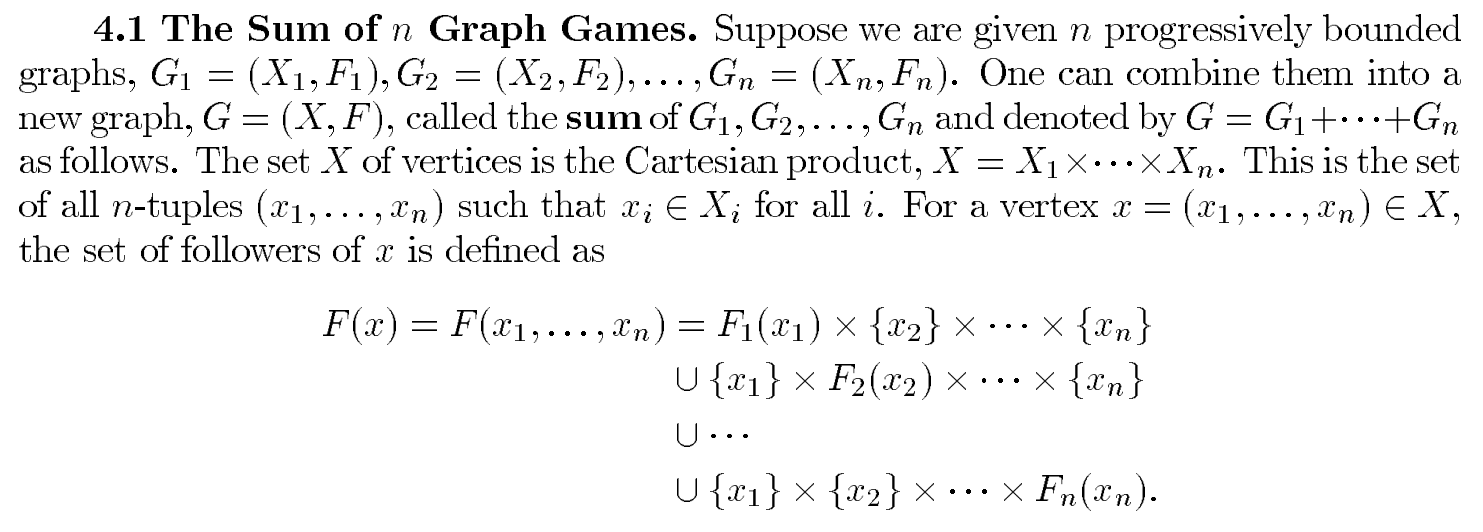
\includegraphics[width=0.5\textwidth,height=0.5\textheight,keepaspectratio]{sumgraph}
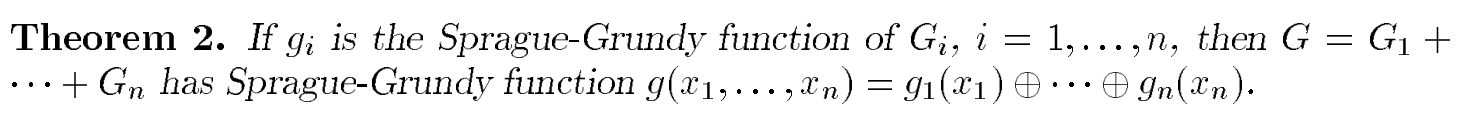
\includegraphics[width=0.5\textwidth,height=0.5\textheight,keepaspectratio]{sgth}
\textbf{Thus}, if a position is a \textbf{N} position, we can cleverly see which position should we go to (what move of a component game to take) such that we reach \textbf {P} position.
\section{Graphs}
\subsection{Tree}
Undirected, acyclic, connected, $|V| - 1$ edges.\\
All edges are bridges, and internal vertices (degree $> 1$) are articulation points.\\
It is as well a bipartite graph.\\
\textbf{SSSP}: Simply take the sum of edge weights of that unique path. $O(|V|)$\\
\textbf{APSP}: Simply do SSSP from all vertices. $O(|V^2|)$
\begin{minted}{cpp}
void preorder (v) {
	visit (v);
	preorder (left (v));
	preorder (right (v));
}
void inorder (v) {
	inorder (left (v));
	visit (v);
	inorder (right (v));
}
void postorder (v) {
	postorder (left (v));
	postorder (right (v));
	visit (v);
}
\end{minted}
It is \textbf {impossible} to construct binary tree with just Preorder traversal.\\ 
It is \textbf {impossible} to construct binary tree with just Inorder traversal.\\
It is \textbf {impossible} to construct binary tree with just Postorder traversal.
\subsubsection{Important Problems}
\begin{itemize}
	\item \href {https://gist.github.com/sourabh2311/6cff69fef833097556696bd6f31f3f1d}{UVA 11695 Sol}: Problem Desc: Find which edge to remove and add so as to minimise the number of hops to travel between flights.\\
	Problem Sol: Just link the center of diameters. Brute force which edge to remove. 
	\item \href {https://github.com/sourabh2311/Competitive-Programming/blob/master/UVA_112.cpp}{UVA 112 Sol}, \href {https://uva.onlinejudge.org/external/1/112.pdf}{UVA 112 Prob}: Just see how I processed the input.	
	\item \href {https://gist.github.com/sourabh2311/6b761c14bef4e5887e6b03b809bc4983}{UVA 10029 Sol}, \href {https://uva.onlinejudge.org/external/100/10029.pdf}{UVA 10029 Prob}: Edit steps, (lexicographic sequence of words)	
	\item \href {https://gist.github.com/sourabh2311/d73572fab5cf6d390f509d29abf4cd60}{UVA 536 Sol}, \href {https://uva.onlinejudge.org/external/5/536.pdf}{UVA 536 Prob}: Construct binary tree with preorder and inorder	
	\item \href {https://gist.github.com/sourabh2311/25edb7a7067948832ade9192bd2635ce}{UVA 10459 Sol}, \href {https://uva.onlinejudge.org/external/104/10459.pdf}{UVA 10459 Prob}: Centers of diameters are best where as corners are worst.	
\end{itemize}
\section{Some Basic}
\begin{minted}{cpp}
	while (first || cin >> temp) {  // something }
\end{minted}
\section{DP}
\subsection{Balanced Bracket Sequence}
A Balanced bracket sequence is a string consisting of only brackets, such that this sequence, when certain numbers and $+$ is inserted gives a valid mathematical expression.
\subsubsection{One type of bracket}
Let depth be the current no. of open brackets, initially depth $= 0$. We iterate over all character of the string; if the current bracket character is an opening bracket then we increment depth, o/w we decrement it. I f at any time the variable depth gets negative, or at the end it is different from 0, then the string is not a balanced sequence otherwise it is.
\subsubsection{MultiType}
Maintain a stack, in chich we will store all opening brackets that we meet. If the current bracket character is an opening one, we put it onto the stack. If it is a closing one, then we check if the stack is non empty, and if the top element is of the same type as the current closing bracket, if both conditions are fulfilled, then we remove the opening bracker from the stack. If at any time one of the ocnditions is not fulfilled or at the end the stack is non empty, then the string is not balanced otherwise it is.
\subsubsection{No. of balanced Sequences}
The number of balanced bracket sequences with only one bracket type can be calculated using the Catalan numbers. The number of balanced bracket sequences of length $2n$ ($n$ pairs of brackets) is: $$\frac{1}{n+1} \binom{2n}{n}$$

If we allow $k$ types of brackets, then each pair be of any of the $k$ types (independently of the others), thus the number of balanced bracket sequences is: $$\frac{1}{n+1} \binom{2n}{n} k^n$$\\
On the other hand these numbers can be computed using dynamic programming. Let $d[n]$ be the number of regular bracket sequences with $n$ pairs of bracket. Note that in the first position there is always an opening bracket. And somewhere later is the corresponding closing bracket of the pair. It is clear that inside this pair there is a balanced bracket sequence, and similarly after this pair there is a balanced bracket sequence. So to compute $d[n]$, we will look at how many balanced sequences of $i$ pairs of brackets are inside this first bracket pair, and how many balanced sequences with $n-1-i$ pairs are after this pair. Consequently the formula has the form: $$d[n] = \sum_{i=0}^{n-1} d[i] \cdot d[n-1-i]$$ The initial value for this recurrence is $d[0] = 1$.
\subsubsection{Lexicographically next balanced sequence}
\begin{minted}{cpp}
	// Idea: "dep" indicates the imbalance in the string s[0...i - 1]. Now after replacing s[i] with ')', dep dec. and we want to add the lexicographically least string having 'dep - 1' closing brackets reserved.
	bool next_balanced_sequence(string & s) {
    int n = s.size();
    int depth = 0;
    for (int i = n - 1; i >= 0; i--) {
        if (s[i] == '(')
            depth--;
        else
            depth++;

        if (s[i] == '(' && depth > 0) {
            depth--;
            int open = (n - i - 1 - depth) / 2;
            int close = n - i - 1 - open;
            string next = s.substr(0, i) + ')' + string(open, '(') + string(close, ')');
            s.swap(next);
            return true;
        }
    }
    return false;
}
\end{minted}
If it is required to find and output all balanced bracket sequences of a specific length $n$.

To generate them, we can start with the lexicographically smallest sequence $((\dots(())\dots))$, and then continue to find the next lexicographically sequences with the algorithm described above. 
\subsubsection{Sequence Index}
Given a balanced bracket sequence with $n$ pairs of brackets. We have to find its index in the lexicographically ordered list of all balanced sequences with $n$ bracket pairs.

Let's define an auxiliary array $d[i][j]$, where $i$ is the length of the bracket sequence (semi-balanced, each closing bracket has a corresponding opening bracket, but not every opening bracket has necessarily a corresponding closing one), and $j$ is the current balance (difference between opening and closing brackets). $d[i][j]$ is the number of such sequences that fit the parameters. We will calculate these numbers with only one bracket type.

For the start value $i = 0$ the answer is obvious: $d[0][0] = 1$, and $d[0][j] = 0$ for $j > 0$. Now let $i > 0$, and we look at the last character in the sequence. If the last character was an opening bracket $($, then the state before was $(i-1, j-1)$, if it was a closing bracket $)$, then the previous state was $(i-1, j+1)$. Thus we obtain the recursion formula: $$d[i][j] = d[i-1][j-1] + d[i-1][j+1]$$ $d[i][j] = 0$ holds obviously for negative $j$. Thus we can compute this array in $O(n^2)$.

Now let us generate the index for a given sequence.

First let there be only one type of brackets. We will us the counter $\text{depth}$ which tells us how nested we currently are, and iterate over the characters of the sequence. If the current character $s[i]$ is equal to $($, then we increment $\text{depth}$. If the current character $s[i]$ is equal to $)$, then we must add $d[2n-i-1][\text{depth}+1]$ to the answer, taking all possible endings starting with a $($ into account (which are lexicographically smaller sequences), and then decrement $\text{depth}$.

New let there be $k$ different bracket types.

Thus, when we look at the current character $s[i]$ before recomputing $\text{depth}$, we have to go through all bracket types that are smaller than the current character, and try to put this bracket into the current position (obtaining a new balance $\text{ndepth} = \text{depth} \pm 1$), and add the number of ways to finish the sequence (length $2n-i-1$, balance $ndepth$) to the answer: $$d[2n - i - 1][\text{ndepth}] \cdot k^{\frac{2n - i - 1 - ndepth}{2}}$$ This formula can be derived as follows: First we "forget" that there are multiple bracket types, and just take the answer $d[2n - i - 1][\text{ndepth}]$. Now we consider how the answer will change is we have $k$ types of brackets. We have $2n - i - 1$ undefined positions, of which $\text{ndepth}$ are already predetermined because of the opening brackets. But all the other brackets ($(2n - i - i - \text{ndepth})/2$ pairs) can be of any type, therefore we multiply the number by such a power of $k$.
\subsubsection{Finding the kth sequence}
Let $n$ be the number of bracket pairs in the sequence. We have to find the $k$-th balanced sequence in lexicographically sorted list of all balanced sequences for a given $k$.

As in the previous section we compute the auxiliary array $d[i][j]$, the number of semi-balanced bracket sequences of length $i$ with balance $j$.

First, we start with only one bracket type.

We will iterate over the characters in the string we want to generate. As in the previous problem we store a counter $\text{depth}$, the current nesting depth. In each position we have to decide if we use an opening of a closing bracket. To put an opening bracket character, it $d[2n - i - 1][\text{depth}+1] \ge k$. We increment the counter $\text{depth}$, and move on to the next character. Otherwise we decrement $k$ by $d[2n - i - 1][\text{depth}+1]$, put a closing bracket and move on.
\begin{minted}{cpp}
	string kth_balanced(int n, int k) {
    vector<vector<int>> d(2*n+1, vector<int>(n+1, 0));
    d[0][0] = 1;
    for (int i = 1; i <= 2*n; i++) {
        d[i][0] = d[i-1][1];
        for (int j = 1; j < n; j++)
            d[i][j] = d[i-1][j-1] + d[i-1][j+1];
        d[i][n] = d[i-1][n-1];
    }

    string ans;
    int depth = 0;
    for (int i = 0; i < 2*n; i++) {
        if (depth + 1 <= n && d[2*n-i-1][depth+1] >= k) {
            ans += '(';
            depth++;
        } else {
            ans += ')';
            if (depth + 1 <= n)
                k -= d[2*n-i-1][depth+1];
            depth--;
        }
    }
    return ans;
}
\end{minted}
Now let there be $k$ types of brackets. The solution will only differ slightly in that we have to multiply the value $d[2n-i-1][\text{ndepth}]$ by $k^{(2n-i-1-\text{ndepth})/2}$ and take into account that there can be different bracket types for the next character.

Here is an implementation using two types of brackets: round and square:
\begin{minted}{cpp}
	string kth_balanced2(int n, int k) {
    vector<vector<int>> d(2*n+1, vector<int>(n+1, 0));
    d[0][0] = 1;
    for (int i = 1; i <= 2*n; i++) {
        d[i][0] = d[i-1][1];
        for (int j = 1; j < n; j++)
            d[i][j] = d[i-1][j-1] + d[i-1][j+1];
        d[i][n] = d[i-1][n-1];
    }

    string ans;
    int depth = 0;
    stack<char> st;
    for (int i = 0; i < 2*n; i++) {
        // '('
        if (depth + 1 <= n) {
            int cnt = d[2*n-i-1][depth+1] << ((2*n-i-1-depth-1) / 2);
            if (cnt >= k) {
                ans += '(';
                st.push('(');
                depth++;
                continue;
            }
            k -= cnt;
        }

        // ')'
        if (depth && st.top() == '(') {
            int cnt = d[2*n-i-1][depth-1] << ((2*n-i-1-depth+1) / 2);
            if (cnt >= k) {
                ans += ')';
                st.pop();
                depth--;
                continue;
            }
            k -= cnt;
        }
            
        // '['
        if (depth + 1 <= n) {
            int cnt = d[2*n-i-1][depth+1] << ((2*n-i-1-depth-1) / 2);
            if (cnt >= k) {
                ans += '[';
                st.push('[');
                depth++;
                continue;
            }
            k -= cnt;
        }

        // ']'
        ans += ']';
        st.pop();
        depth--;
    }
    return ans;
}
\end{minted}
\section{Strings}
To map keyboard etc, it is better to create 2 strings then loop through and map.\\
To transform complete string to lowercase: 
\begin{minted}{cpp} 
transform (word.begin (), word.end (), word.begin (), ::tolower); 
\end{minted}
To concatenate two vectors: 
\begin{minted}{cpp}
vector1.insert (vector1.end (), vector2.begin (), vector2.end ()); 
\end{minted}
\begin{minted}{cpp} 
string.substr (startposn, length); // Where startposn is 0 indexed.
\end{minted}
\begin{minted}{cpp}
int pos1 = line.find ("U=");
if (pos1 != -1) { // process }  
line.replace (pos, len, newString); // pos = line.find (f), len = f.size ()
\end{minted}
We can iterate through all substrings of string $O(n^2)$ and see which all of them are palindromes in $O(n^3)$ or in $O(n^2)$ by using dp ($dp[startpos][endpos] = (s[startpos] == s[endpos] \&\& dp[startpos + 1][endpos - 1]$) or hash.
\subsection{Minimum Edit Distance}
\begin{minted}{cpp}
void fillmem() {
   for (int j = 0; j <= a.size(); j++) mem[0][j] = j;
   for (int i = 0; i <= b.size(); i++) mem[i][0] = i;
   for (int i = 1; i <= b.size(); i++) {
       for (int j = 1; j <= a.size(); j++) {
           if (a[j - 1] == b[i - 1]) mem[i][j] = mem[i - 1][j - 1];
           else mem[i][j] = min(mem[i - 1][j - 1], min(mem[i - 1][j], mem[i][j - 1])) + 1;
       }
   }
    // mem[b.size ()][a.size ()] contains the answer
}
void print() {
   int i = b.size(), j = a.size();
   while (i || j) {
       if (i and j and a[j - 1] == b[i - 1]) { i--; j--; continue; }
       if (i and j and mem[i][j] == mem[i - 1][j - 1] + 1) {
           cout << "C" << b[i - 1]; if (j <= 9) cout << "0";
           cout << j;
           i--; j--;
           continue;
       }
       if (i and mem[i][j] == mem[i - 1][j] + 1) {
           cout << "I" << b[i - 1];
           if (j <= 9) cout << "0";
           cout << j + 1;
           i--;
           continue;
       }
       else if (j) {
           cout << "D" << a[j - 1];
           if (j <= 9) cout << "0";
           cout << j;
           j--;
       }
   }
   cout << "E\n";
}
\end{minted}
\subsection{Length of longest Palindrome possible by removing 0 or more characters}
\begin{minted}{cpp}
dp[startpos][endpos] = s[startpos] == s[endpos] ? 2 + dp[startpos + 1][endpos - 1] : max (dp[startpos + 1][endpos], dp[startpos][endpos - 1])
\end{minted}
\subsection{Longest Common Subsequence}
\begin{minted}{cpp}
memset (mem, 0, sizeof (mem));
for (int i = 1; i <= b.size (); i++) {
	for (int j = 1; j <= a.size (); j++) {
		if (b[i - 1] == a[j - 1]) mem[i][j] = mem[i - 1][j - 1] + 1;
		else mem[i][j] = max (mem[i - 1][j], mem[i][j - 1])
	}
}
void printsol (int ui, int li) {
	ui--; li--;
	vector<string> ans;
	while (ui || li) {
		if (a[ui] == b[li]) {
			ans.push_back (a[ui]);
			ui--; li--;
			continue;
		}
		if (ui and mem[ui][li] == mem[ui - 1][li]) {
			ui--;
			continue;
		}
		if (li and mem[ui][li] == mem[ui][li - 1]) {
			li--;
			continue;
		}
	}
	reverse (ans.begin (), ans.end ());
	cout << ans << "\n";
}
\end{minted}
\subsection{Prefix Function and KMP}
\subsubsection{Prefix Function}
The prefix function for this string is defined as an array $\pi$ of length n, where $\pi[i]$ is the length of the longest proper prefix of the substring $s[0 … i]$ which is also a suffix of this substring. A proper prefix of a string is a prefix that is not equal to the string itself. By definition, $\pi[0]=0$. Example:\\
$abcabchejfabcabca$\\
$00012300001234564$\\
\textbf{Note: } $\pi[i + 1] \leq \pi[i] + 1$ as if $\pi[i + 1] > \pi[i] + 1$ then consider this suffix ending at position i + 1 \& having length $\pi[i + 1]$ - removing the last character we get a suffix ending in position i \& having length $\pi[i + 1] - 1$ that is better than $\pi[i]$. Should be able to reason the following code.
\begin{minted}{cpp}
vector<int> prefix_function(string &s) {  // O(n)
    int n = (int)s.length();
    vector<int> pi(n, 0);
    for (int i = 1; i < n; i++) {
        int j = pi[i-1];
        while (j > 0 && s[i] != s[j])
            j = pi[j-1];
        if (s[i] == s[j])
            j++;
        pi[i] = j;
    }
    return pi;
}
\end{minted}
\subsubsection{KMP}
Given a text t and a string s, we want to find and display the positions of all occurrences of the string s in the text t.
\\For convenience we denote with n the length of the string s and with m the length of the text t.\\
We generate the string s+\#+t, where \# is a separator that doesn't appear in s and t. Let us calculate the prefix function for this string. Now think about the meaning of the values of the prefix function, except for the first n+1 entries (which belong to the string s and the separator). By definition the value π[i] shows the longest length of a substring ending in position i that coincides with the prefix. But in our case this is nothing more than the largest block that coincides with s and ends at position i. This length cannot be bigger than n due to the separator. But if equality π[i]=n is achieved, then it means that the string s appears completely in at this position, i.e. it ends at position i. Just do not forget that the positions are indexed in the string s+\#+t.\\
Thus if at some position i we have π[i]=n, then at the position $i − (n + 1) − n + 1 = i − 2n$ in the string t the string s appears.\\
As already mentioned in the description of the prefix function computation, if we know that the prefix values never exceed a certain value, then we do not need to store the entire string and the entire function, but only its beginning. In our case this means that we only need to store the string s+\# and the values of the prefix function for it. We can read one character at a time of the string t and calculate the current value of the prefix function.
\begin{minted}{cpp}
void kmp() {
    auto pref = prefix_function(p);
    int j = 0;
    int cnt = 0;
	// Note: pi[n] = 0, hence j = 0.
    for (int i = 0; i < t.size(); i++) {
        while (j > 0 and t[i] != p[j]) {
            j = pref[j - 1];
        }
        if (t[i] == p[j]) j++;
        if (j == p.size()) {  // j == n, that means we must dec. j. 
		// And remember that if s[0...n - 1] == s[1...n - 1]s[n-1] that means s[0] = s[1], s[1] = s[2], s[n-2] = s[n-1]. That means all characters are same and hence we haven't lost anything as pref[n - 1] = n - 1.
            cnt++;  // occurence found
            j = pref[j - 1];
        }
    }
}
\end{minted}
\subsubsection{Counting number of occurrences of each prefix}
\begin{minted}{cpp}
vector<int> ans(n + 1);
for (int i = 0; i < n; i++)  // Longest prefix is favored and will have correct count. But remember that longest prefix also have smaller prefix in it. So here i is string index
    ans[pi[i]]++;
for (int i = n-1; i > 0; i--)  // here i is prefix length. Thus we are doing backward propagation
    ans[pi[i-1]] += ans[i];
for (int i = 0; i <= n; i++)  // as only intermediate strings were considered, we didn't consider original prefix.
    ans[i]++;
\end{minted}
\subsection{Notes}
\begin{itemize}
	\item In case of hashing a string, we follow polynomial rolling hash function, with p as a prime number roughly equal to the size of character domain and m as a huge prime number.
	\item If s is palindrome and if $s[0...n - 2]$ is palindrome, that means all characters are same thus if all characters are not same then the longest non palindromic substring is $s[0...n - 2]$ or $s[1...n - 1]$
\end{itemize}
\subsection{SAM}
A suffix automaton for a given string s is a minimal DFA that accepts all the suffixes of the string s.
\begin{itemize}
	\item A suffix automaton is an oriented acyclic graph.
	\item One of the states $t_0$ is the initial state
	\item All transitions originating from a state must have different labels
	\item One or multiple states are marked as terminal states. If we start from the initial state $t_0$ and move along transitions to a terminal state, then the labels of the passed transitions must spell one of the suffixes of the string s. Each of the suffixes of s must be spellable using a path from $t_0$ to a terminal state.
\end{itemize}
Consider any non-empty substring t of the string s. We will denote with endpos(t) the set of all positions in the string s, in which the occurrences of t end. For instance, we have endpos("bc")= \{2,4\} for the string "abcbc".\\
We will call two substrings t1 and t2 endpos-equivalent, if their ending sets coincide i.e. endpos(t1) = endpos(t2). Thus all non-empty substrings of the string s can be decomposed into several equivalence classes according to their sets endpos.\\
It turns out, that in a suffix machine endpos-equivalent substrings correspond to the same state. In other words the number of states in a suffix automaton is equal to the number of equivalence classes among all substrings, plus the initial state.\\
Lemma 1: Two non-empty substrings u and w (with length(u) ≤ length(w)) are endpos-equivalent, if and only if the string u occurs in s only in the form of a suffix of w. (Proof is obvious)\\
Lemma 2: Consider two non-empty substrings u and w (with length(u) ≤ length(w)). Then their sets endpos either don't intersect at all, or endpos(w) is a subset of endpos(u). And it depends on if u is a suffix of w or not. (Proof is obvious)\\
Lemma 3: Consider an endpos-equivalence class. Sort all the substrings in this class by non-increasing length. Then in the resulting sequence each substring will be one shorter than the previous one, and at the same time will be a suffix of the previous one. In other words the substrings in the same equivalence class are actually each others suffixes, and take all possible lengths in a certain interval [x;y].\\
Consider some state v ≠ $t_0$ in the automaton. As we know, the state v corresponds to the class of strings with the same endpos values. And if we denote by w the longest of these strings, then all the other strings are suffixes of w. \textbf{suffix link} \textit{link(v)} leads to the state that corresponds to the longest suffix of w that is another endpos-equivalent class.\\
Lemma 4: Suffix links form a tree with the root $t_0$.\\
Lemma 5: If we build a endpos tree from all the existing sets (according to the principle “the set-parent contains as subsets of all its children”), then it will coincide in structure with the tree of suffix references. \textbf{Note: }$endpos(t_0) = \{-1, 0, \dots, length(s)-1\}$\\
Note: For each state v one or multiple substrings match. We denote by longest(v) the longest such string, and through len(v) its length. We denote by shortest(v) the shortest such substring, and its length with minlen(v). Then all the strings corresponding to this state are different suffixes of the string longest(v) and have all possible lengths in the interval [minlength(v);len(v)]. For each state v ≠ $t_0$ a suffix link is defined as a link, that leads to a state that corresponds to the suffix of the string longest(v) of length $minlen(v) − 1$. minlen(v) = len(link(v))+1 \\
Number of states in suffix automaton of the string s of length n doesn't exceed $2n - 1$ (for n $\geq$ 2)\\
Number of transitions $\leq 3n - 4$.
\begin{minted}{cpp}
#include<bits/stdc++.h>

using namespace std;

typedef pair<int, int> ii;
typedef long long int int;
//Learning in depth about suffix automaton.
struct state {
    int len, link;
    map<char,int> next;
    int cnt;
    int firstpos;
    bool is_clon;
    vector<int> inv_link;
};
const int MAXLEN = 250005;
vector<state> st;
int sz, last;
vector<vector<int> > tcntdata;
vector<int> nsubs, d, lw;
vector<bool> isterminal;
void sa_init(unsigned int size) {
    nsubs.assign(2 * size, 0);
    isterminal.assign(2 * size, false);
    tcntdata.clear();
    tcntdata.resize(2 * size);
    lw.assign(2 * size, 0);
    d.assign(2 * size, 0);
    st.clear();
    st.resize(2 * size);
    sz = last = 0;
    st[0].len = 0;
    st[0].cnt = 0;
    st[0].link = -1;
    st[0].firstpos = -1;
    st[0].is_clon = false;
    ++sz;
    tcntdata[0].push_back(0);
}
void sa_extend (char c) {
    int cur = sz++;
    st[cur].cnt = 1;
    st[cur].len = st[last].len + 1;
    st[cur].firstpos = st[cur].len - 1;
    st[cur].is_clon = false;
    tcntdata[st[cur].len].push_back(cur);
    int p;
    for (p=last; p!=-1 && !st[p].next.count(c); p=st[p].link)
        st[p].next[c] = cur;
    if (p == -1) // In case we came to the root, every non-empty suffix of string sc is accepted by state cur hence we can make link(cur) = t0 and finish our work on this step.
        st[cur].link = 0;
    else {  // Otherwise we found such state q`, which already has transition by character c. It means that all suffixes of length ≤ len(q`) + 1 are already accepted by some state in automaton hence we don’t need to add transitions to state new anymore. But we also have to calculate suffix link for state new.
        int q = st[p].next[c];
        if (st[p].len + 1 == st[q].len)  // The largest string accepted by this state will be suffix of sc of length len(q`) + 1. It is accepted by state t at the moment, in which there is transition by character c from state q`. But state t can also accept strings of bigger length. So, if len(t) = len(q`) + 1, then t is the suffix link we are looking for. We make link(cur) = t and finish algorithm.
            st[cur].link = q;
        else {
            int clone = sz++;
            st[clone].len = st[p].len + 1;
            st[clone].next = st[q].next;
            st[clone].link = st[q].link;
            st[clone].cnt = 0;
            st[clone].firstpos = st[q].firstpos;
            st[clone].is_clon = true;
            tcntdata[st[clone].len].push_back(clone);
            for (; p!=-1 && st[p].next[c]==q; p=st[p].link)
                st[p].next[c] = clone;
            st[q].link = st[cur].link = clone;
        }
    }
    last = cur;
}
// A state v will correspond to set of endpos equivalent strings, cnt[v] will give the number of occurences of such strings
void processcnt() {
    int maxlen = st[last].len;
    for(int i = maxlen; i >= 0; i--) {
        for(auto v : tcntdata[i]) {
            st[st[v].link].cnt += st[v].cnt;
        }
    }
}

// Clearly suffixes should be marked as terminal
void processterminal() {
    isterminal[last] = true;
    int p = st[last].link;
    while(p != -1) {
        isterminal[p] = true;
        p = st[p].link;
    }
}

// Gives the number of substrings (not necessarily distinct). Clearly it should return n.(n+1)/2
int processnumsubs(int at) {
    if(nsubs[at] != 0) return nsubs[at];
    nsubs[at] = st[at].cnt;
    for(auto to : st[at].next) {
        nsubs[at] += processnumsubs(to.second);
    }
    return nsubs[at];
}

void constructSA(string ss) {
    sa_init(ss.size());
    for(int i = 0; i < ss.size(); i++) {
        sa_extend(ss[i]);
    }
    processterminal();
    processcnt();
    for (int v = 1; v < sz; ++v)
        st[st[v].link].inv_link.push_back(v);
    processnumsubs(0);
}
// ---------------------------------------After SA Construction
//
int getcorrstate(string &tosearch) {
    int at = 0;
    for (int i = 0; i < tosearch.size(); i++) {
        if (!st[at].count (tosearch[i])) return -1;
        at = st[at].next[tosearch[i]];
    }
    return at;
}

bool exist(string &tosearch) {
    int at = getcorrstate (tosearch);
    return at == -1 ? false : true;
}

// Returns number of different substrings = number of paths in DAG. And number of paths is clearly not a function of number of states in DAG.
// d[v] = 1 + summation (d[w])
int numdiffsub(int at) {
    if(d[at] != 0) return d[at];
    d[at] = 1;
    for(auto to : st[at].next) {
        d[at] += numdiffsub(to.second);
    }
    return d[at];
}

// Returns total length of all distinct substrings = summation_path (number of edges constituting that path) in DAG.
// ans[v] = summation (d[w] + ans[w]) basically, once we know ans[w], we know that we have number of paths starting from that node + ans[w] // as we know that in each of the contributing strings we should add 1 for this character transition as this character occurs in path for reaching this state. Plus 1 as to consider this character on its own.
int totlength(int at) {
    if(lw[at] != 0) return lw[at];
    for(auto to : st[at].next) {
        lw[at] += d[to.second] + totlength(to.second);
    }
    return lw[at];
}

// Find Lexicographically K-th Substring (here repeated substring is allowed):
void kthlexo(int at, int k, string &as) {
    if(k <= 0) return;
    for(auto to : st[at].next) {
        if(nsubs[to.second] >= k) {
            as.push_back(to.first);
            kthlexo(to.second, k - st[to.second].cnt, as);
            break;
        } else {
            k -= nsubs[to.second];
        }
    }
}
// Repeated substring not allowed
void kthlexo2(int at, int k, string &as) {
    if(k <= 0) return;
    for(auto to : st[at].next) {
        if(d[to.second] >= k) {
            as.push_back(to.first);
            kthlexo2(to.second, k - 1, as);
            break;
        } else {
            k -= d[to.second];
        }
    }
}
// Returns true is the given string is the suffix of T
bool issuffix(string &tosearch) {
    int at = getcorrstate (tosearch);
    return isterminal[at];
}

// Returns how many times P enters in T (occurences can overlap)
/* for each state v of the machine calculate a number 'cnt[v]' which is equal to the
 * size of the set endpos(v). In fact, all the strings corresponding to the same state
 * enter the T same number of times which is equal to the number of positions in the set
 * endpos. */
int numoccur(string &tosearch) {
    int at = getcorrstate (tosearch);
    return at == -1 ? 0 : st[at].cnt;
}

// Return position of the first occurrence of substring in T
int firstpos(string &tosearch) {
    int at = getcorrstate (tosearch);
    return st[at].firstpos - tosearch.size() + 1;
}

// Returns Positions of all occurrences of substring in T
void output_all_occurences (int v, int P_length) {
    if (!st[v].is_clon)
        cout << st[v].firstpos - P_length + 1 << "\n";
    for (size_t i=0; i<st[v].inv_link.size(); ++i)
        output_all_occurences(st[v].inv_link[i], P_length);
}

void smallestcyclicshift(int n) {
    int at = 0;
    string anss;
    int length = 0;
    while(length != n) {
        for (auto it : st[at].next) {
            anss.push_back(it.first);
            at = it.second;
            length++;
            break;
        }
    }
    cout << anss << "\n";
    // cout << st[at].firstpos - n + 1 << "\n"; may give the index for that shift.
}


int main() {
    string s;
    cin >> s;
    constructSA(s);
    int choice;
    cout << "Choose your option:\n1: Substring exist in T or not\n2: Number of different substring of T\n";
    cout << "3: To find total length of distinct substrings\n";
    cout << "4: To check whether the given string is suffix or not\n";
    cout << "5(5.1): To print the K-th lexicographic substring (Repeated substrings allowed)\n";
    cout << "6: To see how many times, given string occurs in T\n";
    cout << "7: To find the position of the first occurrence of substring in T\n";
    cout << "8: To find position of all the occurences of substring in T\n";
    cout << "9(5.2): To print the K-th lexicographic substring (Repeated substrings not allowed)\n";
    cout << "10: To find the smallest cyclic shift\n";

    cout << "15: to exit\n";
    cin >> choice;
    if(choice == 15) break;
    string ss, ns;
    int k, v;
    switch(choice) {
        case 1:
            cout << "Enter your string\n";
            cin >> ss;
            if (exist(ss)) {
                cout << "yes it exist\n";
            } else {
                cout << "no it does not exist\n";
            }
            //cout << "Enter new to string to search for\n";
            break;
        case 2:
            cout << numdiffsub(0) - 1 << "\n";
            break;
        case 3:
            numdiffsub(0);
            cout << totlength(0) << "\n";
            break;
        case 4:
            cout << "Enter the string\n";
            cin >> ss;
            if(issuffix(ss)) cout << "yes\n";
            else cout << "no\n";
            break;
        case 5:
            cin >> k;
            ss.clear();
            kthlexo(0, k, ss);
            if(ss.empty()) {
                ss = "No such line.";
            }
            cout << ss << "\n";
            break;
        case 6:
            cout << "Enter string\n";
            cin >> ss;
            cout << numoccur(ss) << "\n";
            break;
        case 7:
            cout << "Enter string\n";
            cin >> ss;
            cout << firstpos(ss) << "\n";
            break;
        case 8:
            cout << "Enter string\n";
            cin >> ss;
            /*for(v = 0; v < s.size(); v++) {
                cout << setw(2) << v;
            }
            cout << "\n";
            for(v = 0; v < s.size(); v++) {
                cout << setw(2) << s[v];
            }
            cout << "\n";*/
            v = getcorrstate(ss);
            if(v != -1) {
                output_all_occurences(v, ss.size());
            }
            break;
        case 9:
            cin >> k;
            numdiffsub(0);
            kthlexo2(0, k, ss);
            if(ss.empty()) {
                ss = "No such line.";
            }
            cout << ss << "\n";
            break;
        case 10:
            cout << "Enter S\n";
            cin >> ss;
            s = ss + ss;
            constructSA(s);
            smallestcyclicshift(ss.size ());
            break;
    }
    return 0;
}
\end{minted}
\subsection{Important Problems}
\textit{Review: cf 631D}
\begin{itemize}
	\item \href {https://github.com/sourabh2311/Competitive-Programming/blob/master/UVA_10739.cpp}{UVA 10739 Sol}, \href {https://uva.onlinejudge.org/external/107/10739.pdf}{UVA 10739 Prob}: String to palindrome, just see the minimum edit distance between this string and its reverse but need to divide by 2 later as both strings are it itself.	
	\item \href {https://codeforces.com/contest/245/problem/H}{Queries for the number of palindromic substrings within given range}, \href {https://github.com/sourabh2311/Competitive-Programming/blob/master/IMP%20QUES/Suffix%20String%20Structure/Hash/514C%20-%20Watto%20And%20Mechanism.cpp}{\textbf {See this soln to see power of hashing.}}: 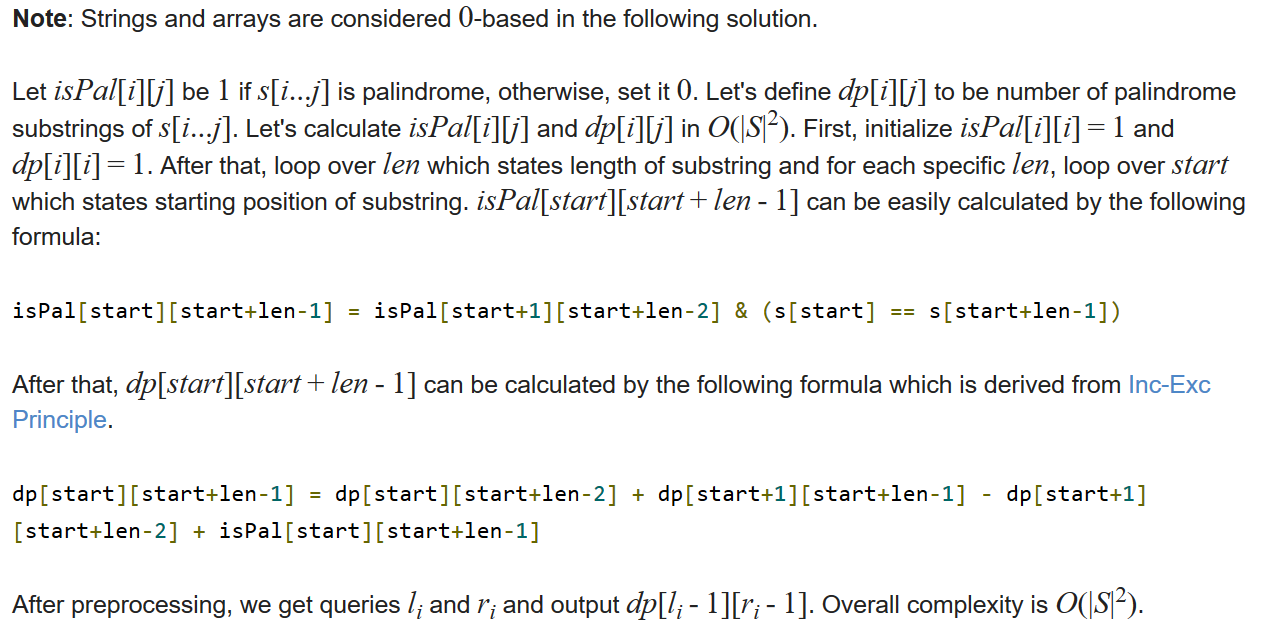
\includegraphics[width=0.5\textwidth,height=0.5\textheight,keepaspectratio]{palsub} 	
	\item \href {https://github.com/sourabh2311/Competitive-Programming/blob/master/HimanshuSA11107.cpp}{UVA 11107 Sol - simple}, \href {https://github.com/sourabh2311/Competitive-Programming/blob/master/HimanshuSA11107.cpp}{UVA 11107 Sol - complicated but more powerful}: Problem is to find the longest substring shared by more than half of given strings.	
	\item \href {https://gist.github.com/sourabh2311/25edb7a7067948832ade9192bd2635ce}{UVA 10459 Sol}, \href {https://uva.onlinejudge.org/external/104/10459.pdf}{UVA 10029 Prob}: Edit steps, (lexicographic sequence of words)	
\end{itemize}
\end{document}
